\section{Dependency Rule Synthesis}\label{sec:alg}

This section describes the \depsynth synthesis algorithm,
which automatically generates a set of dependency rules
that are sufficient to guarantee crash consistency for a set of litmus tests.
It formalizes the dependency rule synthesis problem,
gives an overview of \depsynth's approach to synthesizing dependency rules,
and then presents the core \depsynth algorithm (\cref{fig:alg:depsynth}).

\subsection{Problem Statement}\label{sec:alg:problem}

\depsynth solves the problem of 
finding a \emph{single} set of dependency rules \ruleset
that makes every litmus test \test
in a set of tests \tests
crash consistent (\cref{def:crash-consistent}).
% As \cref{sec:problem:tests} discusses,
% the set of tests \tests of interest
% can be drawn from a number of sources,
% including hand-written tests
% and automated fuzzing or enumeration.
%
While \cref{def:crash-consistent} suffices to find a set of rules \ruleset
that guarantees crash consistency,
it does not rule out \emph{cyclic} solutions that cannot be executed on real hardware.
For example, consider a program $P$
where $\evaluate{P}{\sys} = [\texttt{write}(a_1, v_1, \langle n_1, t_1 \rangle), \texttt{write}(a_2, v_2, \langle n_2, t_2 \rangle)]$.
The set of rules $R = \{ \deprule{n_1}{n_2}{=}, \deprule{n_2}{n_1}{=} \}$
makes $P$ crash consistent.
These two rules do not admit any valid crash schedules
other than the trivial $\vec{s} = \vec{\top}$ and $\vec{s} = \vec{\bot}$ schedules,
as \cref{def:valid-schedule} forces $s_1 = s_2$.
In effect, crash consistency for $P$
requires both writes to happen ``at the same time''.
But on real disks the level of write atomicity is only a single data block,
so there is no way for both writes to happen at the same time.
To rule out cyclic solutions,
we follow the example of happens-before graphs~\cite{lamport:happens-before}
from distributed systems and memory consistency,
and require the set of synthesized dependency rules \ruleset to be \emph{acyclic}.\tighten

\subsection{The \depsynth Algorithm}\label{sec:alg:alg}

\begin{figure}
    \centering
    {\xsmall\begin{algorithmic}[1]
\Function{\depsynthalg}{\impl, \tests, \consist}
\State $\ruleset \gets \{\}$
\Loop
    \State $\test \gets \Call{NextTest}{\tests, \ruleset, \impl, \consist}$  \label{alg:depsynth:nexttest}
    \If{$\test = \bot$}  \Comment{\ruleset makes all tests in \tests crash consistent}
        \State \Return \ruleset
    \EndIf
    \State $\tests \gets \tests \setminus \test$
    \State $\ruleset' \gets \Call{\rulesfortest}{\test, \impl, \consist}$ \label{alg:depsynth:rulesone}
    \If{$\ruleset' = \bot$}
        \State \Return \UNSAT  \Comment{No rules can make \test crash consistent}
    \EndIf
    \State $\ruleset \gets \ruleset \cup \ruleset'$ \label{alg:depsynth:add}
    \If{$\neg \Call{Acyclic}{\ruleset}$}  \Comment{Fail if new rules create a cycle in the rule set}
        \State \Return \UNKNOWN  \label{alg:depsynth:resolve}
    \EndIf
\EndLoop
\EndFunction

\vspace{0.8em}

\Function{NextTest}{\tests, \ruleset, \impl, \consist}
    \For{$\test \in \tests$}
        \If{$\neg \Call{\crashconsistentalg}{\test, \ruleset, \impl, \consist}$}
            \State \Return \test
        \EndIf
    \EndFor
    \State \Return $\bot$
\EndFunction

\vspace{0.8em}

\Comment{Check Def.~\ref{def:crash-consistent} with an SMT solver}
\Function{\crashconsistentalg}{$\test = \langle P_\emph{initial}, P_\emph{main} \rangle$, \ruleset, \impl, \consist}  \label{alg:depsynth:cc}
    \State $d_\emph{initial} \gets \run{\evaluate{P_\emph{initial}}{\mathcal{O}}}{\vec{\top}}{d_0}$
    \State \Return $\forall \vec{s}.\ \valid{\vec{s}}{P_\emph{main}}{R} \Rightarrow \consistent{\run{\evaluate{P_\emph{main}}{\mathcal{O}}}{\vec{s}}{d_\emph{initial}}}$
\EndFunction

\algstore{depsynth}
\end{algorithmic}
}
    \caption{The \depsynth algorithm takes as input a storage system implementation $\sys$,
    a set of litmus tests \tests, and a crash-consistency predicate $\textrm{\emph{Consistent}}$,
    and returns an acyclic set of dependency rules that make all tests in \tests crash consistent (\cref{def:crash-consistent}).
    The search synthesizes dependency rules for one litmus test at a time.
    If the rules generated for two or more tests result in a cycle,
    this algorithm fails; \cref{sec:alg:cycles} discusses an extension for continuing 
    the search for an acyclic solution.}
    \label{fig:alg:depsynth}
\end{figure}

The \depsynthalg algorithm (\cref{fig:alg:depsynth})
takes as input a storage system implementation \sys,
a set of litmus tests \tests,
and a crash-consistency predicate $\emph{Consistent}$.
Given these inputs,
it synthesizes a set of dependency rules
that is acyclic and sufficient to make all tests \tests crash consistent.
% \depsynth delegates rule generation to
% a \textsc{RulesForTests} subprocedure (\cref{sec:alg:onetest})
% that takes as input a single test $\test$,
% evaluates it into a set of write operations $\{ w_i \}$,
% and searches for a minimal happens-before graph over those writes
% that is sufficient to ensure crash consistency.
% Once it identifies such a happens-before graph,
% it uses a simple syntactic approach
% to generalize it into a set of dependency rules
% that suffice to enforce the orderings in the graph.

\depsynthalg does not try to generate a sufficient set of dependency rules
for all tests in \tests at once,
since this would require a prohibitively expensive search
over large happens-before graphs.
Instead, it works incrementally:
at each iteration of its top-level loop,
\depsynthalg chooses a single test \test that is not made crash consistent
by the current candidate set of dependency rules (line~\ref{alg:depsynth:nexttest} in \cref{fig:alg:depsynth}), 
invokes the procedure \rulesfortest (\cref{sec:alg:onetest})
to synthesize dependency rules that make \test crash consistent,
and adds the new rules to the candidate set (line~\ref{alg:depsynth:add}).
Working incrementally reduces the number of litmus tests
for which \depsynthalg needs to synthesize rules;
for example, in \cref{sec:eval:shardstore} we show that only \shardstoretestsused of \shardstoreinputtests tests
were passed to \rulesfortest to synthesize a sufficient set of dependency rules
for a production key-value store.
This reduction relieves developers from being selective about the set of litmus tests they supply to \depsynth,
and makes it possible to, for example, use the output of a fuzzer or random test generator as input.

However, because the rules for each test are generated independently,
it is possible for the union of the generated rules to contain a cycle---%
even if the rules for each individual test do not---%
and so be an invalid solution (\cref{sec:alg:problem}).
The algorithm in \cref{fig:alg:depsynth}
returns \UNKNOWN if such a cycle is found.
We have not seen this failure mode occur for the storage systems we evaluated (\cref{sec:eval}),
but it is possible in principle.
In \cref{sec:alg:cycles}, we explain how to extend \depsynthalg
to recover from cycles by generalizing \rulesfortest to synthesize rules for multiple tests at once.

\depsynthalg delegates checking for crash consistency
to the procedure \crashconsistentalg (line~\ref{alg:depsynth:cc}), 
which takes as input a single litmus test
and a set of dependency rules,
and checks whether the rules make the test crash consistent
according to \cref{def:crash-consistent}.
This procedure uses symbolic evaluation of the storage system implementation \sys
to generate the logical encoding described in \cref{sec:problem:crashes},
and solves the resulting formulas using an off-the-shelf SMT solver~\cite{niemetz:boolector}.\tighten

\subsection{Synthesizing Dependency Rules with Happens-Before Graphs}\label{sec:alg:onetest}

\begin{figure}
    \centering
    {\xsmall\begin{algorithmic}[1]
\algrestore{depsynth}

\Function{\rulesfortest}{$\test = \langle P_\emph{initial}, P_\emph{main} \rangle$, \impl, \consist}
    \State $\wr \gets \{w\ | \ w \in \evaluate{P_\emph{main}}{\impl} \}$
    \State \Return $\Call{\phaseone}{\tests, [], \wr, \impl, \consist}$
\EndFunction

\vspace{0.8em}

\Function{\phaseone}{\test, \ord, \wr, \impl, \consist}  \Comment{Search for total orders over writes}  \label{fig:rules:phase1}
    \If{$\wr = \emptyset$}
        \State $\gr \gets \{ (\ord[i], \ord[j]) \ | \ 0 \leq i < j < |\ord| \}$
        \State \Return \Call{\phasetwo}{\tests, \gr, \impl, \consist}  \Comment{\gr is a total order; minimize it in Phase 2} \label{fig:rules:phase1tophase2}
    \EndIf
    \For{$w \in \wr$}
        \State $\ord' \gets \ord + [w]$
        \State $\wr' \gets \wr \setminus \{ w \}$
        \State $\gr \gets \{ (\ord[i], \ord[j]) \ | \ 0 \leq i < j < |\ord| \} \, \cup$ 
            \Statex $\hspace{6em}\{ (w_1, w_2) \ | \ w_1 \in \ord \land w_2 \in \wr \} \, \cup$ 
            \Statex $\hspace{6em}\{ (w_1, w_2) \ | \ w_1, w_2 \in \wr \}$  \label{fig:rules:phase1angelic}
         \If{$\neg \crashconsistentalg(\test, \Call{\rulesforgraph}{\gr}, \impl, \consist)$}  \label{fig:rules:phase1sufficient}
            \State \textbf{continue} \label{fig:rules:phase1continue}
        \EndIf
        \State $\ruleset \gets \Call{\phaseone}{\test, \ord', \wr', \impl, \consist}$
        \If{$\ruleset \neq \bot$}
            \State \Return \ruleset
        \EndIf
    \EndFor
    \State \Return $\bot$
\EndFunction

\algstore*{depsynth}
\end{algorithmic}
}
    \caption{The algorithm for generating sufficient dependency rules for a litmus test \test
    searches the space of happens-before graphs over the writes performed by \test.
    The first phase searches for total orders over the writes that are sufficient for crash consistency.
    Once such a total order is found, the second phase removes edges from it until the happens-before graph is minimal.}
    \label{fig:alg:rulesfortests}
\end{figure}

\begin{figure}
    \centering
    {\xsmall\begin{algorithmic}[1]
\algrestore{depsynth}

\Function{\rulesforgraph}{\gr}  \Comment{Generalize a happens-before graph into dependency rules}  \label{fig:rules:rulesforgraph}
    \State $\ruleset \gets \{\}$
    \For{$(w_1, w_2) \in \gr$}
        \State $\langle n_1, t_1 \rangle \gets \Call{Label}{w_1}$  \Comment{Get label $l_1 = \langle n_1, t_1 \rangle$ for write $w_1 = \texttt{write}(a_1, s_1, l_1)$}
        \State $\langle n_2, t_2 \rangle \gets \Call{Label}{w_2}$
        \If{$t_1 < t_2$}
            \State $\ruleset \gets \ruleset \cup \{ \deprule{n_2}{n_1}{>} \}$  \Comment{Invert the order, as a rule $\deprule{n_a}{n_b}{p}$ says $n_a$ happens \textbf{after} $n_b$}
        \ElsIf{$t_1 = t_2$}
            \State $\ruleset \gets \ruleset \cup \{ \deprule{n_2}{n_1}{=} \}$
        \Else
            \State $\ruleset \gets \ruleset \cup \{ \deprule{n_2}{n_1}{<} \}$
        \EndIf
    \EndFor
    \State \Return \ruleset
\EndFunction 

\algstore*{depsynth}
\end{algorithmic}
}
    \caption{The procedure for generalizing a happens-before graph \gr into dependency rules
    constructs (at most) one rule for each edge.}
    \label{fig:alg:rulesforgraph}
\end{figure}

The core of the \depsynthalg algorithm is the
\rulesfortest procedure in \cref{fig:alg:rulesfortests},
which takes as input a litmus test \test,
a storage system implementation $\sys$,
and a crash-consistency predicate $\emph{Consistent}$,
and synthesizes a set of dependency rules
that makes \test crash consistent.
\rulesfortest frames the rule synthesis problem
as a search over \emph{happens-before graphs}~\cite{lamport:happens-before}
on the writes performed by the test.
An edge $(w_1, w_2)$ between two writes in a happens-before graph
says that write $w_1$ must persist to disk before write $w_2$.
Happens-before graphs and dependency rules have a natural correspondence:
if a happens-before graph includes an edge $(w_1, w_2)$,
a dependency rule $\deprule{n_2}{n_1}{p}$ that matches the writes' labels
is sufficient to enforce the required ordering.
\rulesfortest searches for a minimal, acyclic happens-before graph
that is sufficient to ensure crash consistency for \test,
and then syntactically generalizes that happens-before graph into a set of dependency rules.

\rulesfortest searches for a happens-before graph by first finding a \emph{total
order} on the writes that makes $T$ crash consistent (\phaseone), and then
searching for a minimal \emph{partial order} within this total order that is
both sufficient for crash consistency and yields an acyclic set of dependency
rules (\phasetwo). The algorithm is exhaustive: it tries all total orders and
all minimal partial orders within a total order, until it finds a solution or
fails because a solution does not exist.

\rulesfortest builds on the observation that crash consistency (\cref{def:crash-consistent})
is monotonic with respect to the subset relation on dependency rules---%
if a set of dependency rules \ruleset is not sufficient for crash consistency,
then no subset of \ruleset is sufficient either:
%
\begin{theorem}[Monotonicity of crash consistency]\label{thm:synthesis:monotonicity}
Let \test be a litmus test
and \ruleset a set of dependency rules for a storage system $\sys$.
If \ruleset does not make \test crash consistent (according to \cref{def:crash-consistent}),
then no subset $R' \subset R$ can make \test crash consistent.
\end{theorem}
\begin{proof}[Proof sketch]
If \ruleset does not make \test crash consistent,
there exists a valid crash schedule $\vec{s}$ (\cref{def:valid-schedule})
that does not satisfy the crash consistency predicate $\emph{Consistent}$.
By \cref{def:valid-schedule}, each rule in \ruleset only adds additional constraints on the possible valid crash schedules.
Removing a rule from \ruleset therefore only allows more valid crash schedules,
and so if $\vec{s}$ was a valid crash schedule for \ruleset, it is also a valid crash schedule for any subset of \ruleset.
\end{proof}
%
\noindent
\rulesfortest applies this property by checking crash consistency
for a happens-before graph \gr before exploring any subgraphs of \gr;
if \gr is not sufficient, then neither is any subgraph of \gr,
and so that branch of the search can be skipped.
% In contrast, a bottom-up search that tries to add new edges to \gr
% cannot be guided by this feedback,
% as knowing that a graph \gr is not sufficient does not give any information
% about whether a larger supergraph of \gr would provide crash consistency.

% As happens-before graphs are directed acyclic graphs,
% \rulesfortest splits the search for a minimal sufficient happens-before graph into two phases---%
% first searching for a candidate total order over the writes,
% and then shrinking that total order into a partial one that still ensures crash consistency.
% This phase split to accelerate the search;
% the first phase can remove many edges from the graph in a single step,
% and so can quickly rule out large portions of the search space,
% while the second phase works one edge at a time.

\paragraph{Total order search.}
\phaseone (line~\ref{fig:rules:phase1})
explores all possible total orders over the writes in \test
that are sufficient for crash consistency.
At each recursive call, the list \ord represents a total order over some of \test's writes,
and the set \wr contains all writes not yet added to that order.
\phaseone tries to add each write in \wr to the end of the total order.
Each time, it checks whether the new total order leads to a crash consistency violation (line~\ref{fig:rules:phase1sufficient})
and if so, prunes this branch of the search.
For \phaseone to be complete, 
this check must behave angellically for the writes in \wr that have not yet been added to the order---%
if there is \emph{any possible} set of dependency rules for the remaining writes that would succeed,
the check must succeed.
We make the check angelic by including every possible dependency rule for the remaining writes (line~\ref{fig:rules:phase1angelic}).
If the test cannot be made crash consistent even with every possible rule included,
then by \cref{thm:synthesis:monotonicity} no subset of those rules
(i.e., formed by completing the rest of the total order)
can succeed either, so the prefix is safe to prune.
\phaseone continues until every write has been added to the total order
and then moves to \phasetwo to further reduce the happens-before graph.\tighten

\paragraph{Partial order search.}
Starting from a happens-before graph \gr that reflects a total order over all writes in \test,
\phasetwo (line~\ref{fig:rules:phase2})
removes edges from the graph until it is minimal,
i.e., removing any further edges would violate crash consistency.
\phasetwo removes one edge at a time from the graph \gr (line~\ref{fig:rules:phase2remove}),
checks if the graph remains sufficient for crash consistency (line~\ref{fig:rules:phase2sufficient}),
and if so, recurses to remove more edges.
By greedily removing one edge at a time,
\phasetwo is guaranteed to find a minimal result,
and because \phasetwo considers removing every possible edge from \gr
(except those that cannot lead by solutions by \cref{thm:synthesis:monotonicity}),
it is complete---if an acyclic solution exists, \phasetwo will reach it.\tighten

\paragraph{Generating rules from happens-before graphs.}
The \rulesfortest search operates on happens-before graphs,
but its goal is to synthesize dependency rules (\cref{def:dependency-rule}).
The \rulesforgraph procedure (\cref{fig:alg:rulesforgraph})
bridges this gap
by taking as input a happens-before graph \gr
and returning a set of dependency rules \ruleset
that are sufficient to enforce the ordering requirements that \gr dictates.
\rulesforgraph uses a simple syntactic approach to generate a rule for each edge in \gr:
if $(w_1, w_2) \in \gr$,
where writes $w_1$ and $w_2$ have labels $l_1 = \langle n_1, t_1 \rangle$ and $l_2 = \langle n_2, t_2 \rangle$, respectively,
then it generates a rule of the form $\deprule{n_2}{n_1}{}$
(reversing the order because $G$ is a happens-before graph
but dependency rules are happens-\emph{after} edges).
To choose an epoch predicate for the generated rule,
we compare the two epochs $t_1$ and $t_2$
and select the predicate that would make the rule match the labels $l_1$ and $l_2$.\tighten

This approach can lead to rules that are too general,
as some rules it generates may only need to apply to certain individual epochs
but will instead apply to all epochs that match the predicate.
Overly general rules risk sacrificing performance
by preventing reordering or caching optimizations that would be safe.
However, this same generality also allows \textsc{RulesForTests} to avoid overfitting to the input litmus tests.
In \cref{sec:eval:shardstore} we show that generated rules generalize well in practice (i.e., are not overfit),
and that they filter out few additional schedules compared to expert-written rules.

\paragraph{Properties of \rulesfortest.}
The \rulesfortest algorithm is \emph{sound}:
all paths that return a solution are guarded by checks of crash consistency and of acyclicity,
and so satisfy the requirements of \cref{sec:alg:problem}.
\rulesfortest is also \emph{complete}:
each of \phaseone and \phasetwo are complete, as discussed above,
and so together form a complete search over the space of total orders. 
Every possible acyclic solution must be a subgraph of some total order,
since the transitive closure of edges in any happens-before graph is a (strict) partial order,
and so exploring all total orders suffices to reach any possible acyclic solution.
Finally, \rulesfortest is \emph{minimal},
in the sense that removing any rule from a returned set \ruleset
would violate crash consistency. 
\phasetwo continues removing edges from a candidate graph \gr
until \cref{thm:synthesis:monotonicity} says it cannot be made smaller,
and is therefore guaranteed to find a minimal happens-before graph. 
Every rule in \ruleset is justified by (at least) one edge in that graph,
and since dependency rules cannot overlap
(in \cref{def:dependency-rule}, the possible epoch predicates are disjoint),
removing any rule would incorrectly allow reordering of its corresponding edge(s).
%\todo{these are long sentences, perhaps we should just do three thms and proof sketches}

\begin{example}\label{sec:alg:example}
Consider running \rulesfortest for the simple log-structured key-value store
and \texttt{SingleEntry_TwoAppend} litmus test from \cref{s:overview}.
From \cref{sec:problem:example} we know that this test produces a set \wr of four writes:
%
\begin{align*}
    w_1 &= \texttt{write}(2, \texttt{to_block}((1, 81)), \langle \textsf{log}, 1 \rangle), \\
    w_2 &= \texttt{write}(0, \texttt{to_block}((1, 3)),  \langle \textsf{superblock}, 1 \rangle), \\
    w_3 &= \texttt{write}(3, \texttt{to_block}((2, 37)), \langle \textsf{log}, 2 \rangle), \\
    w_4 &= \texttt{write}(0, \texttt{to_block}((1, 4)),  \langle \textsf{superblock}, 2 \rangle)
\end{align*}
%
\phaseone first chooses the first write to add to the total order.
Suppose it chooses $w_2$.
This choice results in the following graph \gr at line~\ref{fig:rules:phase1angelic}
(shaded nodes are in \ord; white nodes are in \wr):
%
\begin{center}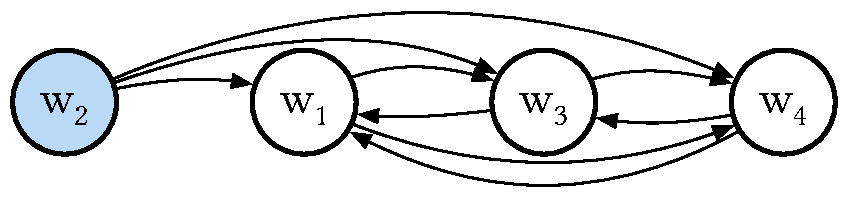
\includegraphics[width=0.5\textwidth]{figs/sec4-1.pdf}\end{center}
%
The check at line~\ref{fig:rules:phase1sufficient}
finds that this graph is not crash consistent: it allows a crash schedule where $w_2$ is on disk but no other writes are,
which violates the crash-consistency predicate as $w_2$ is a superblock write pointing to a log block that is not on disk.
\phaseone therefore continues (line~\ref{fig:rules:phase1continue}),
which prunes any total order that starts with $[w_2]$ from the search,
and chooses a next write to consider, say $w_3$.
The total order starting with $[w_3]$ does pass the crash consistency check,
so \phaseone recurses with $\ord = [w_3]$ and $\wr = \{w_1, w_2, w_4\}$.
In this recursive call,
suppose we again first choose $w_2$ to add to the total order.
This choice results in the following graph \gr:
%
\begin{center}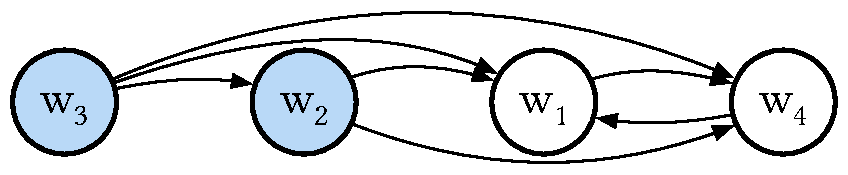
\includegraphics[width=0.5\textwidth]{figs/sec4-2.pdf}\end{center}
%
Again, line~\ref{fig:rules:phase1sufficient} finds that this graph is not crash consistent,
for the same reason as before (superblock write $w_2$ can be on disk when log write $w_1$ is not),
and so the search continues, pruning any total order that starts with $[w_3, w_2]$.
Suppose it next chooses $w_1$ to add to the total order.
This choice succeeds, making the recursive call with $\ord = [w_3, w_1]$ and $\wr = \{w_2, w_4\}$.
From here, any choice \phaseone makes will succeed.
Supposing it choses $w_2$ first,
\phaseone eventually reaches line~\ref{fig:rules:phase1tophase2} and continues to \phasetwo
with the following initial graph \gr:
%
\begin{center}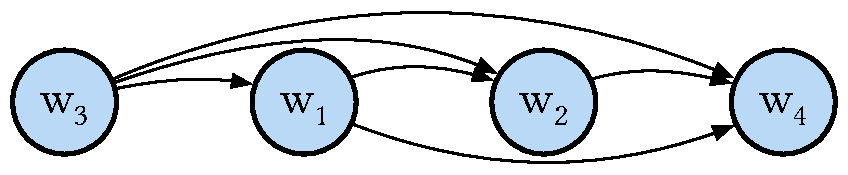
\includegraphics[width=0.5\textwidth]{figs/sec4-3.pdf}\end{center}

\phasetwo proceeds by trying to remove one edge at a time from \gr.
Suppose it first chooses to remove edge $(w_3, w_1)$,
and so recurses at line~\ref{fig:rules:phase2recurse} on the graph $\gr' = \gr \setminus \{(w_3, w_1)\}$.
This graph still ensures crash consistency at line~\ref{fig:rules:phase2sufficient},
as writing $w_1$ before $w_3$ does not affect consistency.
The recursion can continue twice more
by choosing and successfully removing edges $(w_3, w_2)$ and then $(w_1, w_4)$ as well,
eventually reaching line~\ref{fig:rules:phase2loop} with the following graph \gr (now with write labels shown):\tighten
%
\begin{center}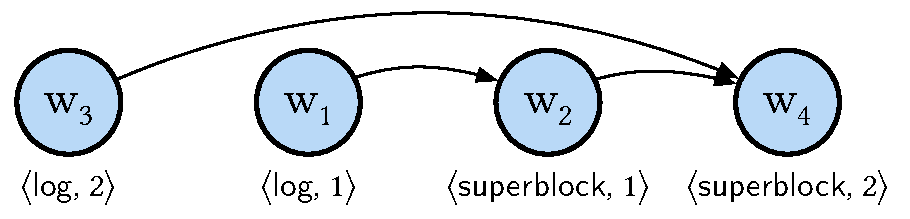
\includegraphics[width=0.5\textwidth]{figs/sec4-4.pdf}\end{center}
%
From here, the loop in \phasetwo now tries to remove each of the three remaining edges,
but each attempted $\gr'$ violates crash consistency and so returns $\bot$ from the next recursive call.
\phasetwo therefore exits the loop with the above graph \gr,
which we now know is minimal as no further edges can be removed.
Applying \rulesforgraph to \gr yields the two rules from \cref{s:overview}:
\begin{align*}
    \deprule{\textsf{superblock}&}{\textsf{log}}{=} & \text{ from edges } (w_3, w_4) \text{ and } (w_1, w_2) \\
    \deprule{\textsf{superblock}&}{\textsf{superblock}}{>} & \text{ from edge } (w_2, w_4).
\end{align*}
\end{example}


\subsection{Resolving Cycles in Dependency Rules}\label{sec:alg:cycles}

% \begin{figure}
%     \centering
%     {\xsmall\newcommand{\impl}{\ensuremath{\mathcal{O}}\xspace}
\newcommand{\test}{\ensuremath{T}\xspace}
\newcommand{\tests}{\ensuremath{\mathcal{T}}\xspace}
\newcommand{\consist}{\ensuremath{\emph{Consistent}}\xspace}
\newcommand{\rulemap}{\ensuremath{\mathcal{R}}\xspace}
\newcommand{\ruleset}{\ensuremath{R}\xspace}
% \newcommand{\writesused}{\ensuremath{W_U}\xspace}
% \newcommand{\writesleft}{\ensuremath{W_R}\xspace}
\renewcommand{\wr}{\ensuremath{W}\xspace}
\newcommand{\ord}{\ensuremath{V}\xspace}
\newcommand{\gr}{\ensuremath{G}\xspace}
\newcommand{\comp}{\ensuremath{C}\xspace}

\begin{algorithmic}[1]
\algrestore{depsynth}

\Function{ResolveCycle}{\rulemap, \impl, \consist}
    \State $C \gets \Call{GetCycle}{\cup_{(T' \mapsto R) \in \rulemap} R}$  \Comment{Identify rules $C \subseteq R$ that participate in the cycle}
    \State $\tests' \gets \{ T \ | \ (T \mapsto R) \in \rulemap \land T \in C \}$  \Comment{Collect the tests that generated rules in $C$}
    \State \Return \Call{RulesForTests}{\tests', \impl, \consist}
\EndFunction

\end{algorithmic}}
%     \caption{The algorithm for resolving cycles in a set of generated dependency rules.
%     \textsc{ResolveCycles} takes as input a mapping from litmus tests to sets of dependency rules
%     such that the union of the sets contains a cycle. It returns a new mapping from the same set of
%     litmus tests to sets of dependency rules that no longer contains a cycle.}
%     \label{fig:alg:resolvecycles}
% \end{figure}

The top-level \depsynthalg algorithm generates rules for each litmus test independently.
Even though the rules generated for each test are guaranteed to be acyclic,
it is possible for the \emph{union} of those rules to contain a cycle,
and so violate the requirements of \cref{sec:alg:problem}.
In practice, we have not seen this happen for the storage systems we evaluate in \cref{sec:eval},
and so the version of \depsynthalg presented in \cref{fig:alg:depsynth} fails if the synthesized rules contain a cycle.

To handle cyclic rules,
\rulesfortest can be extended to support synthesizing rules for multiple litmus tests at once.
This extension adds the writes from \emph{all} the tests into the set of writes \wr,
searches for a total order over that entire set in \phaseone,
and then searches for a minimal happens-before graph over the entire set in \phasetwo.
Edges between writes from different tests
cannot influence the crash consistency of individual tests
(in \cref{def:valid-schedule} they will just lead to spurious additional implications),
and they will eventually be removed by \phasetwo,
creating a forest of disjoint happens-before graphs.
\phasetwo is therefore guaranteed to return an acyclic set of dependency rules
for all the tests it was provided.

In the limit, \depsynthalg could just invoke \rulesfortest with its entire input set \tests,
but this would be prohibitively expensive for any non-trivial set of tests.
Instead, our implementation resolves cycles in \depsynthalg
by identifying which individual litmus tests caused the cycle
(i.e., which tests the rules in the cycle were generated from),
and passes only that subset of tests to the extended \rulesfortest.
